%==============================================
\subsection{W–Clearance Connectivity Graph (WCCG)}
\label{subsec:wccg}
\begin{figure*}[t]
  \centering
  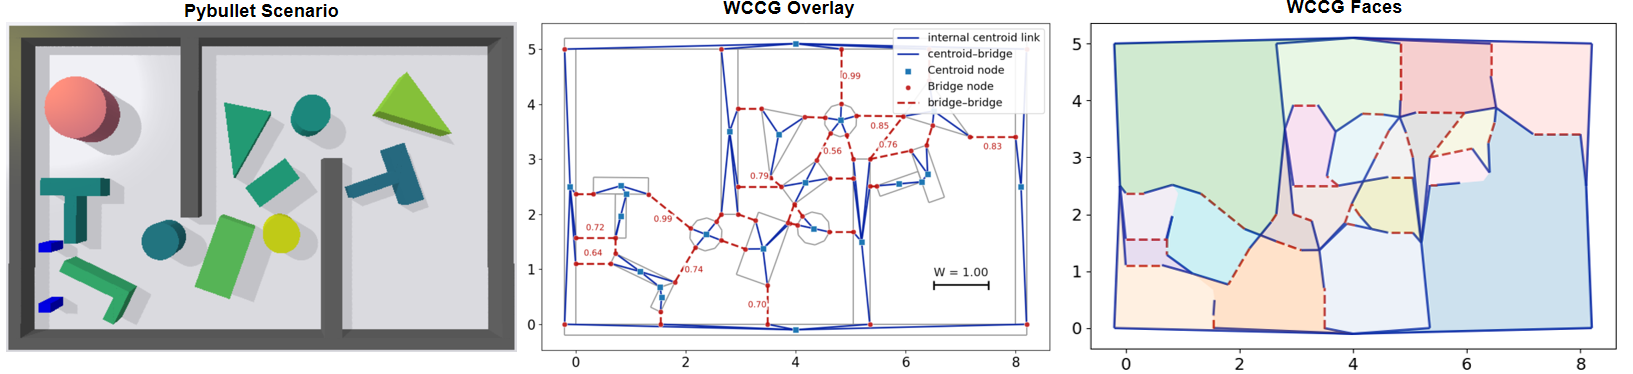
\includegraphics[width=\linewidth]{figures/wccg.pdf}
  \vspace{-3mm}
  \caption{(Left) top–down scene; (Middle) W–CCG with centroid (blue) and bridge (red) nodes, red dashed edges encode gaps $<W$; (Right) faces induced by W–CCG.}
  \label{fig:wccg}
  \vspace{-4mm}
\end{figure*}

To reason about the existence of a traversable corridor of width~$W$, we construct a
\emph{W–Clearance Connectivity Graph} (WCCG) that captures obstacle–to–obstacle
adjacency under the threshold~$W$ and supports fast connectivity queries between
start $\mathbf{s}^{\texttt{S}}$ and goal $\mathbf{s}^{\texttt{G}}$.

\subsubsection{Construction (high level).}
Polygonal obstacles are convex–decomposed. For each convex part we add a
\emph{centroid} node; for each visible closest pair between two parts whose distance
is $<W$, we add \emph{bridge} nodes at the closest points and a bridge–bridge edge
annotated by the gap width; centroid–bridge edges connect bridges to their parts.
Red dashed edges (Fig.~\ref{fig:wccg}) mark \emph{narrow gaps}.

\subsubsection{Connectivity test.}\label{subsubsec:bugplanner}
We employ a ray–shoot and loop–follow routine (“BugPlanner”) on the WCCG frontiers:
from a current point we shoot toward the goal, walk the encountered frontier loop by
angular order, and either reach $\mathbf{s}^{\texttt{G}}$ or certify a blocking
loop. If connected, the routine returns a \emph{skeleton} (an ordered
center–bridge–center sequence) witnessing that $\mathbf{s}^{\texttt{S}}$ and
$\mathbf{s}^{\texttt{G}}$ lie in the same face of the induced decomposition.

\begin{theorem}[Complete criterion for a $W$–clear path]
\label{thm:complete-W-test}
Let $\mathcal{F}_W := \mathbb{R}^2 \setminus (\mathcal{O}\oplus \mathbb{B}_{W/2})$
be the $W$–clear free space. A collision–free path of clearance at least $W$
exists between $\mathbf{s}^{\texttt{S}}$ and $\mathbf{s}^{\texttt{G}}$ iff
(i) they lie in the same face of the WCCG induced by $\mathcal{F}_W$, and
(ii) both endpoint disks $\mathbb{B}_{W/2}(\mathbf{s}^{\texttt{S}})$ and
$\mathbb{B}_{W/2}(\mathbf{s}^{\texttt{G}})$ are obstacle–free.
\end{theorem}

\noindent\textit{Proof sketch.}
BugPlanner yields a frontier \emph{skeleton} within one face.
By convex decomposition and angular–order, each center–bridge–center segment
can be slid onto the boundary of the $W/2$–inflated obstacles without touching
unintended parts; concatenating these slides forms a boundary–following curve with
cross–gap hops. A small inward offset lies entirely in $\mathcal{F}_W$; with cleared
endpoint disks, short connectors attach the endpoints, giving a geometric $W$–clear
path. The converse is immediate.

\begin{remark}[Practical check]
In code we simply (a) run WCCG connectivity; (b) verify the two $W/2$ endpoint disks.
If (a) passes but (b) fails, a few \emph{away–from–endpoint} pushes may clear the disks;
this is an engineering add–on, not core to the method.
\end{remark}


\begin{algorithm}[t]
\small
\caption{BugPlanner for $W$-width connectivity (skeleton witness)}
\label{alg:bugplanner}
\DontPrintSemicolon
\SetKwInOut{Input}{In}\SetKwInOut{Output}{Out}
\Input{$\mathbf{s}^{\texttt{S}}$, $\mathbf{s}^{\texttt{G}}$, WCCG}
\Output{if connected: skeleton $\Sigma$; else: frontier loop $\mathcal{L}$}
$P\leftarrow\mathbf{s}^{\texttt{S}}$, $\Sigma\leftarrow[\ ]$\;
\While{true}{
  \If{segment $P\mathbf{s}^{\texttt{G}}$ hits no edge}{\Return $\Sigma \cup \{\texttt{straight}(P,\mathbf{s}^{\texttt{G}})\}$}
  Build loop $\mathcal{L}$ by angle-follow from the hit edge; append traversed edges to $\Sigma$\;
  \If{$\mathrm{parity}(\mathcal{L},\,\mathbf{s}^{\texttt{S}}\mathbf{s}^{\texttt{G}})$ is odd}{\Return $(\emptyset,\mathcal{L})$}
  Choose exit $e$ on $\mathcal{L}$ (outward normal $\to\,\mathbf{s}^{\texttt{G}}$); append arc to $\Sigma$; $P\leftarrow e$ (tiny bias)\;
}
\end{algorithm}

\begin{remark}[Skeleton $\to$ path]
BugPlanner certifies connectivity via a frontier skeleton. A geometric $W$–clear path is obtained by sliding $\Sigma$ onto the $W/2$–inflated boundary, offsetting slightly inward into $\mathcal F_W$, and attaching the cleared endpoint disks. This mapping is continuous and preserves homotopy.
\end{remark}